
\documentclass[conference,letterpaper]{IEEEtran}
\usepackage[T1]{fontenc}
\usepackage{mathptmx}
\usepackage{graphicx}
\usepackage{amsmath}
\usepackage{tabularx}
\usepackage{float}
\usepackage{balance}
\usepackage{listings}
\usepackage{url}
\usepackage[hidelinks]{hyperref}
\lstset{basicstyle=\ttfamily\scriptsize,breaklines=true,columns=fullflexible,keepspaces=true,showstringspaces=false,frame=single,framerule=0.2pt,xleftmargin=3pt,xrightmargin=3pt}
\hyphenation{ware-house re-plen-ish-ment}
\begin{document}
\title{Smart Warehouse Intelligence}
\author{\IEEEauthorblockN{Ankith Ramesh Babu}\IEEEauthorblockA{Independent Operations Analytics Project}}
\maketitle
\thispagestyle{plain}\pagestyle{plain}
\begin{abstract}This paper presents a reproducible inventory-reconciliation and replenishment analysis using 5,760 synthetic observations from four warehouses and twelve stock-keeping units over 120 days. Daily ERP and WMS snapshots identify 2,245 discrepancy observations, while demand fulfillment reaches 99.56\%. A separate decision table applies a 28-day demand window, fixed lead time and an illustrative safety-stock rule. Two closing-snapshot proposals total 469 units. Increasing lead time from three to fourteen days changes proposals from 280 to 836 units. Offline dashboards, editable Power BI project source and automated tests support auditability. The work evaluates internally consistent analytical rules, not an executed inventory policy.\end{abstract}

\begin{IEEEkeywords}inventory reconciliation, replenishment, safety stock, warehouse analytics, reproducibility\end{IEEEkeywords}

\section{Introduction and System Architecture}

\subsection{Questions addressed}

\textbullet{} Where do ERP and WMS snapshots disagree?


\textbullet{} How much demand remains unfulfilled?


\textbullet{} Which warehouse-SKU pairs cross the reorder threshold?


\textbullet{} How sensitive are proposals to assumed lead time?


\subsection{Processing sequence}

Table~\ref{tab:1} summarizes analysis stages and outputs.

\begin{table}[H]
\caption{Analysis stages and outputs}\label{tab:1}
\centering\footnotesize
\setlength{\tabcolsep}{3pt}
\begin{tabularx}{\columnwidth}{>{\raggedright\arraybackslash}X >{\raggedright\arraybackslash}X >{\raggedright\arraybackslash}X}
\hline
\textbf{Stage} & \textbf{Implementation} & \textbf{Output} \\
\hline
Generate & Seeded Python simulation & Operational records \\
Calculate & Documented business rules & KPIs and decision fields \\
Export & Deterministic CSV / JSON writer & Auditable report files \\
Present & HTML and PBIR visual definitions & Interactive review surfaces \\
Verify & Unit tests, schema and browser checks & Validation evidence \\
\hline
\end{tabularx}
\end{table}

\subsection{Design decisions}

The analysis uses Python standard-library functions to keep execution portable. The browser report embeds its data and needs no server. The Power BI model embeds the same CSV snapshot in Power Query, avoiding machine-specific paths. Data generation and decision rules remain separate from presentation.


\subsection{Operational boundaries}

This is a batch analysis of simulated observations. It does not write to SAP, execute procurement transactions, reserve stock or authorize operational changes. Each exported row retains the identifiers needed to trace a result back to its source observation.


\section{Data specification and provenance}

All source observations are generated in src/run.py with a fixed random seed \cite{r1}. No customer, supplier or employee data is used. Regional names represent four analytical groups, not actual sites.


Table~\ref{tab:2} summarizes source fields and definitions.

\begin{table}[H]
\caption{Source fields and definitions}\label{tab:2}
\centering\footnotesize
\setlength{\tabcolsep}{3pt}
\begin{tabularx}{\columnwidth}{>{\raggedright\arraybackslash}X >{\raggedright\arraybackslash}X >{\raggedright\arraybackslash}X}
\hline
\textbf{Field} & \textbf{Type} & \textbf{Meaning} \\
\hline
warehouse + sku + day & Composite key & 4 warehouses x 12 SKUs x 120 days \\
opening\_stock & Integer & Previous ERP closing stock \\
received & Integer & Sampled from 0, 0, 0, 0, 30, 50 \\
demand & Integer & Daily demand sampled from 2 to 22 \\
shipped & Integer & min(opening stock + receipts, demand) \\
erp\_stock & Integer & Opening + received - shipped \\
wms\_stock & Integer & max(0, ERP stock + sampled noise) \\
variance & Integer & WMS minus ERP stock \\
\hline
\end{tabularx}
\end{table}

Each warehouse-SKU series starts with 120 to 500 ERP units. WMS noise is sampled from -3, 0, 0, 0, 2. Stock observations are snapshots, so totals across dates are not an inventory balance. Seed 43 produces the baseline. Simulation days are numbered periods, not calendar dates.


\subsection{Traceability}

Committed CSVs, KPI JSON, analysis JSON and the Power BI embedded snapshot refer to the same default run. Changes to seeds or assumptions require regenerated reports and a new result interpretation.


\section{Analytical Methodology}

Table~\ref{tab:3} summarizes metric definitions.

\begin{table}[H]
\caption{Metric definitions}\label{tab:3}
\centering\footnotesize
\setlength{\tabcolsep}{3pt}
\begin{tabularx}{\columnwidth}{>{\raggedright\arraybackslash}X >{\raggedright\arraybackslash}X}
\hline
\textbf{Calculation} & \textbf{Rule} \\
\hline
History window & Latest 28 observations per warehouse-SKU \\
Demand variability & Sample standard deviation (n - 1) \cite{r2} \\
Safety stock & 1.65 x standard deviation x sqrt(lead time) \\
Reorder point & ceil(mean demand x lead time + safety stock) \\
Target stock & ceil(mean demand x 21 target days + safety stock) \\
Trigger & Latest WMS stock <= reorder point \\
Proposal & max(target stock - WMS stock, 0), only when triggered \\
\hline
\end{tabularx}
\end{table}

\subsection{Worked example}

At mean demand 12 units/day, standard deviation 4 and lead time 7 days, the reorder point is ceil(84 + 17.46) = 102 units. The 21-day target is 270. Stock of 90 triggers a proposal for 180 units. Stock of 120 does not trigger an order, even though it is below target.


\subsection{Decision timing}

Proposals use the final day after closing stock is known. They do not feed back into the receipt simulation. This is a decision snapshot, not a tested replenishment policy. The z value is illustrative and does not establish achieved service probability.


\section{Results and interpretation}

The analysis output is shown in Fig.~\ref{fig:results}.

\begin{figure}[!t]
\centering
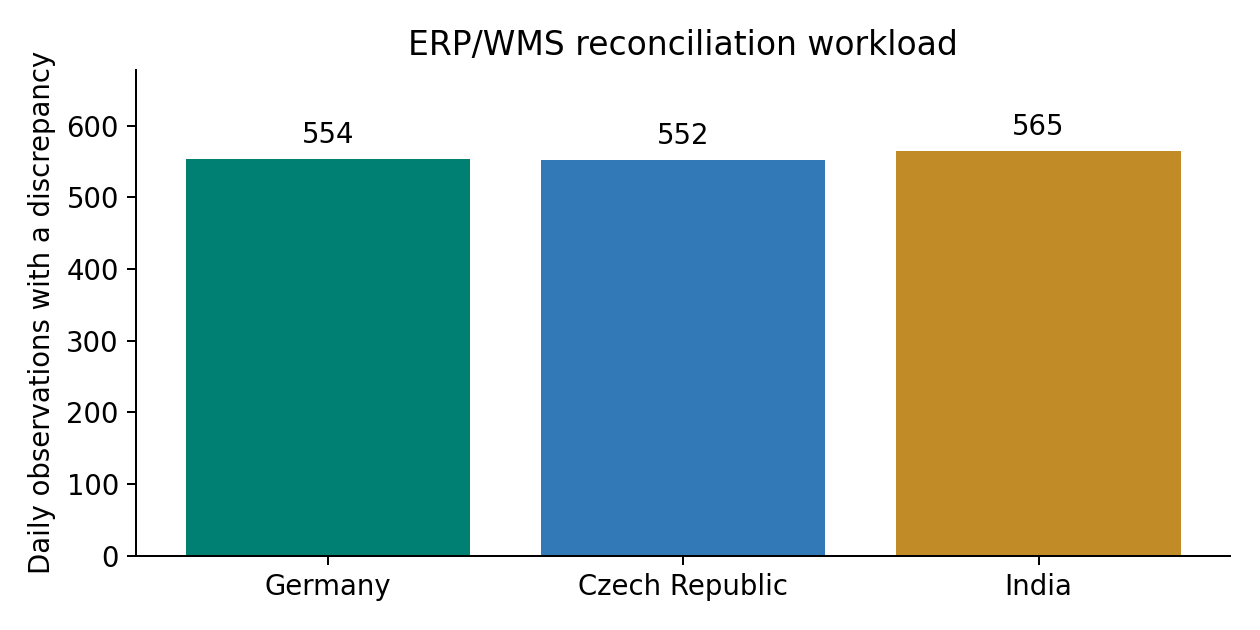
\includegraphics[width=\columnwidth,height=0.25\textheight,keepaspectratio]{../../reports/figures/results.png}
\caption{Baseline results calculated from the committed operational records.}\label{fig:results}
\end{figure}

Table~\ref{tab:4} summarizes regional baseline results.

\begin{table}[H]
\caption{Regional baseline results}\label{tab:4}
\centering\footnotesize
\setlength{\tabcolsep}{3pt}
\begin{tabularx}{\columnwidth}{>{\raggedright\arraybackslash}X >{\raggedright\arraybackslash}X >{\raggedright\arraybackslash}X >{\raggedright\arraybackslash}X}
\hline
\textbf{Warehouse} & \textbf{Discrepancies} & \textbf{Demand} & \textbf{Shipped} \\
\hline
Germany & 554 & 17,523 & 17,371 \\
Hong Kong & 552 & 17,470 & 17,316 \\
Taiwan & 565 & 17,444 & 17,444 \\
Malaysia & 574 & 17,196 & 17,196 \\
\hline
\end{tabularx}
\end{table}

The dataset contains 306 unfulfilled demand units. High aggregate fulfillment does not remove SKU-level risk: Germany SKU005 ends at zero WMS stock and receives a 290-unit proposal. Germany SKU002 receives 179 units. Both final proposal rows have zero ERP/WMS variance.


The 2,245 discrepancy count describes noisy observations across time, not 2,245 distinct damaged items or stock-loss events. Repeated observations of a SKU must not be interpreted as independent physical losses.


\section{Interactive dashboard overview}

The dashboard view is shown in Fig.~\ref{fig:dashboard}.

\begin{figure*}[!t]
\centering
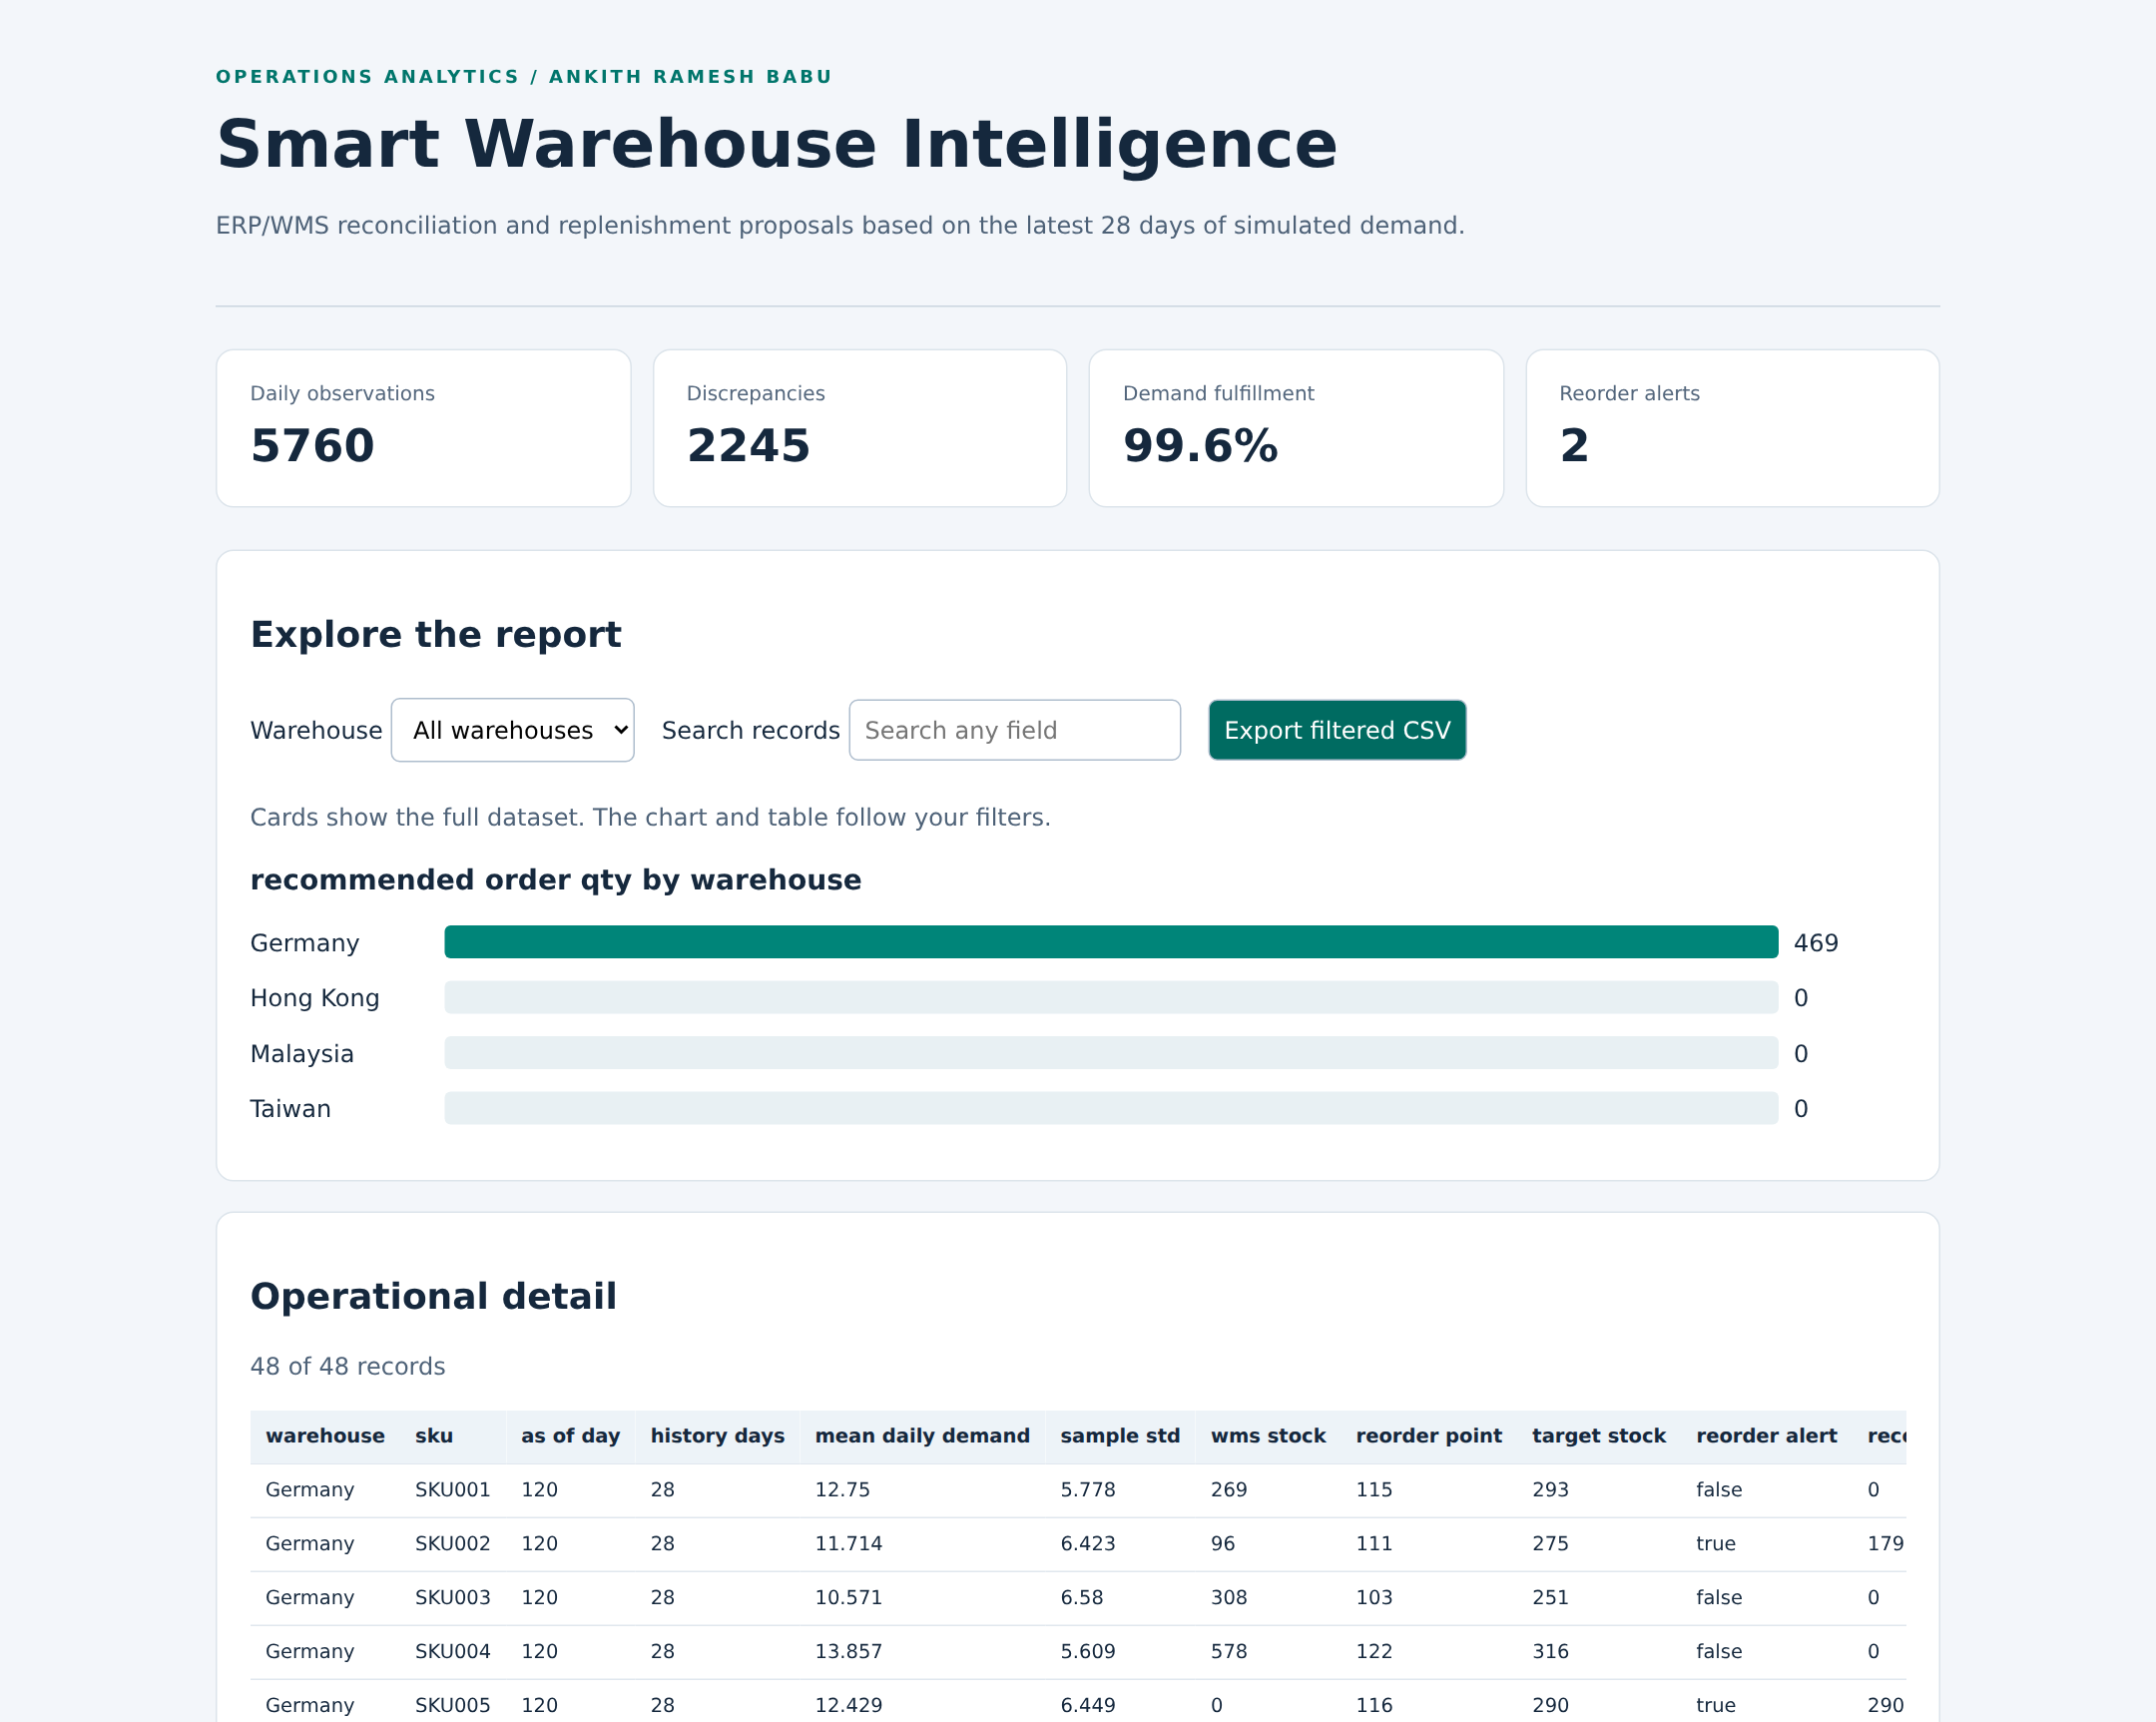
\includegraphics[width=0.90\textwidth,height=0.72\textheight,keepaspectratio]{../../reports/figures/dashboard.png}
\caption{Actual browser capture of the generated HTML dashboard, baseline run.}\label{fig:dashboard}
\end{figure*}

The overview combines full-dataset KPI cards with warehouse filtering, text search, a comparative bar chart and a detailed register. Its data is embedded in the HTML, so the report opens offline without account access.


Display precision differs from the calculation exports: the HTML KPI cards show one decimal place for ratios, while KPI JSON preserves four decimal places. This is display rounding, not a calculation difference.


\section{Dashboard interaction and audit trail}

The dashboard view is shown in Fig.~\ref{fig:reconciliation}.

\begin{figure*}[!t]
\centering
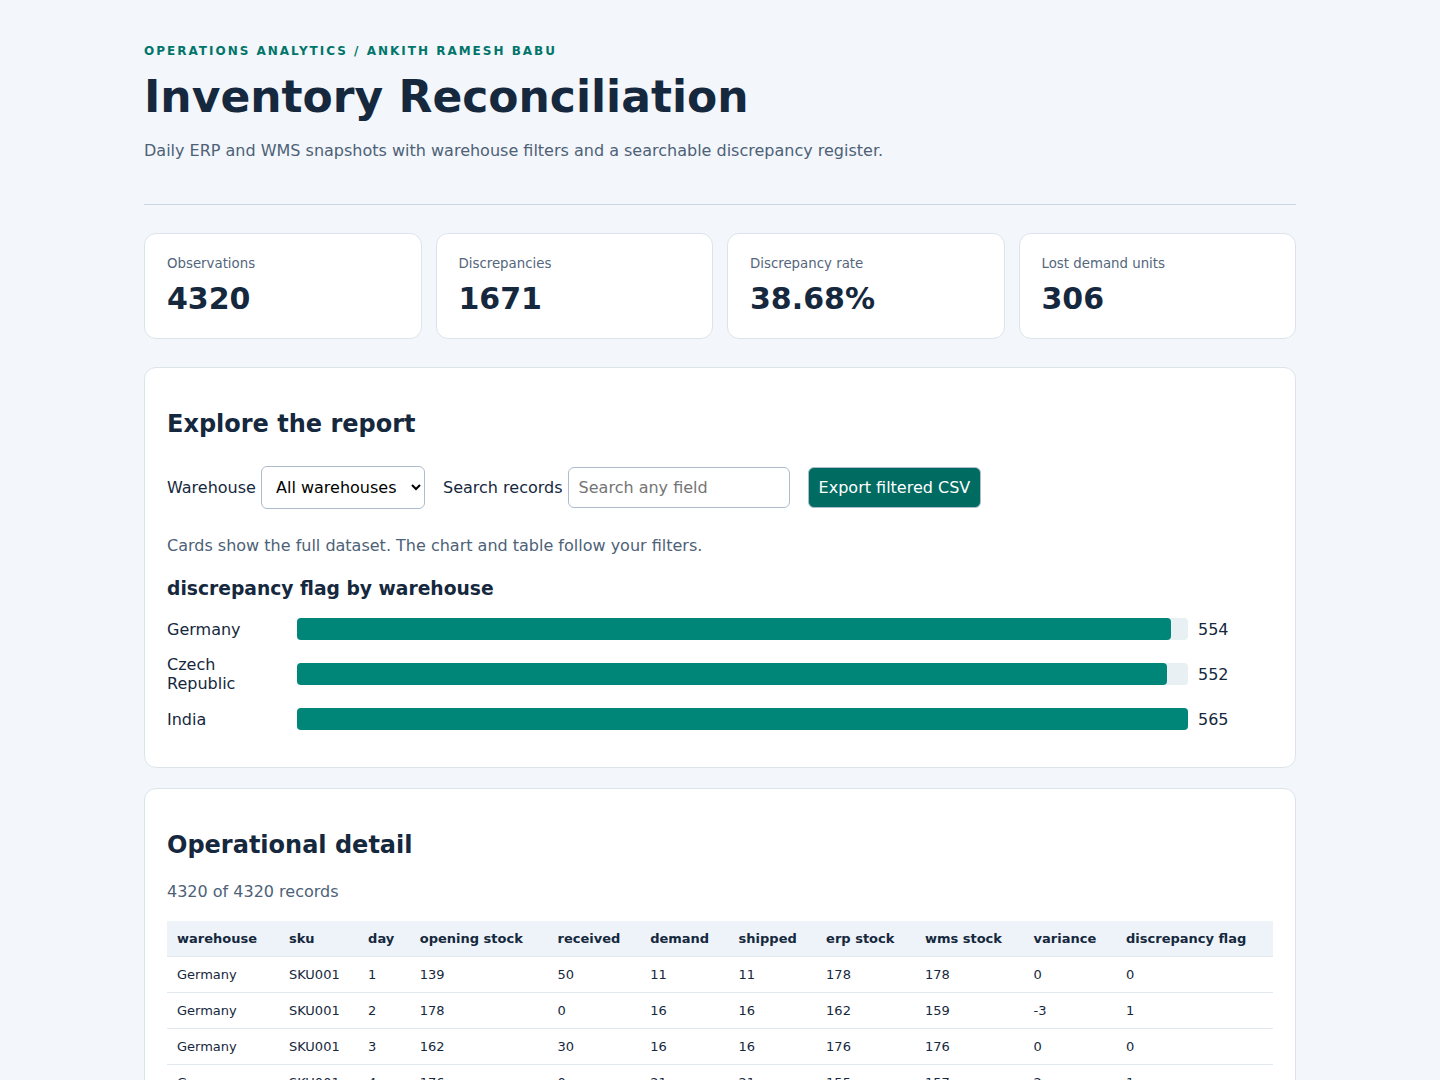
\includegraphics[width=0.90\textwidth,height=0.72\textheight,keepaspectratio]{../../reports/figures/reconciliation.png}
\caption{Actual browser capture of the daily inventory reconciliation view.}\label{fig:reconciliation}
\end{figure*}

Warehouse and search filters update the chart and visible detail rows. Summary cards intentionally remain scoped to the complete dataset. The table displays at most 200 matching rows for responsiveness. CSV export includes every matching row, not only the displayed sample.


In the browser checks, selecting Germany returned records, an unmatched search returned zero rows, and filtered CSV download succeeded. The layout also passed a 390-pixel mobile-width overflow check. The wide detail table remains horizontally scrollable.


\section{Power BI model and page layout}

The report layout is shown in Fig.~\ref{fig:powerbi-layout}.

\begin{figure*}[!t]
\centering
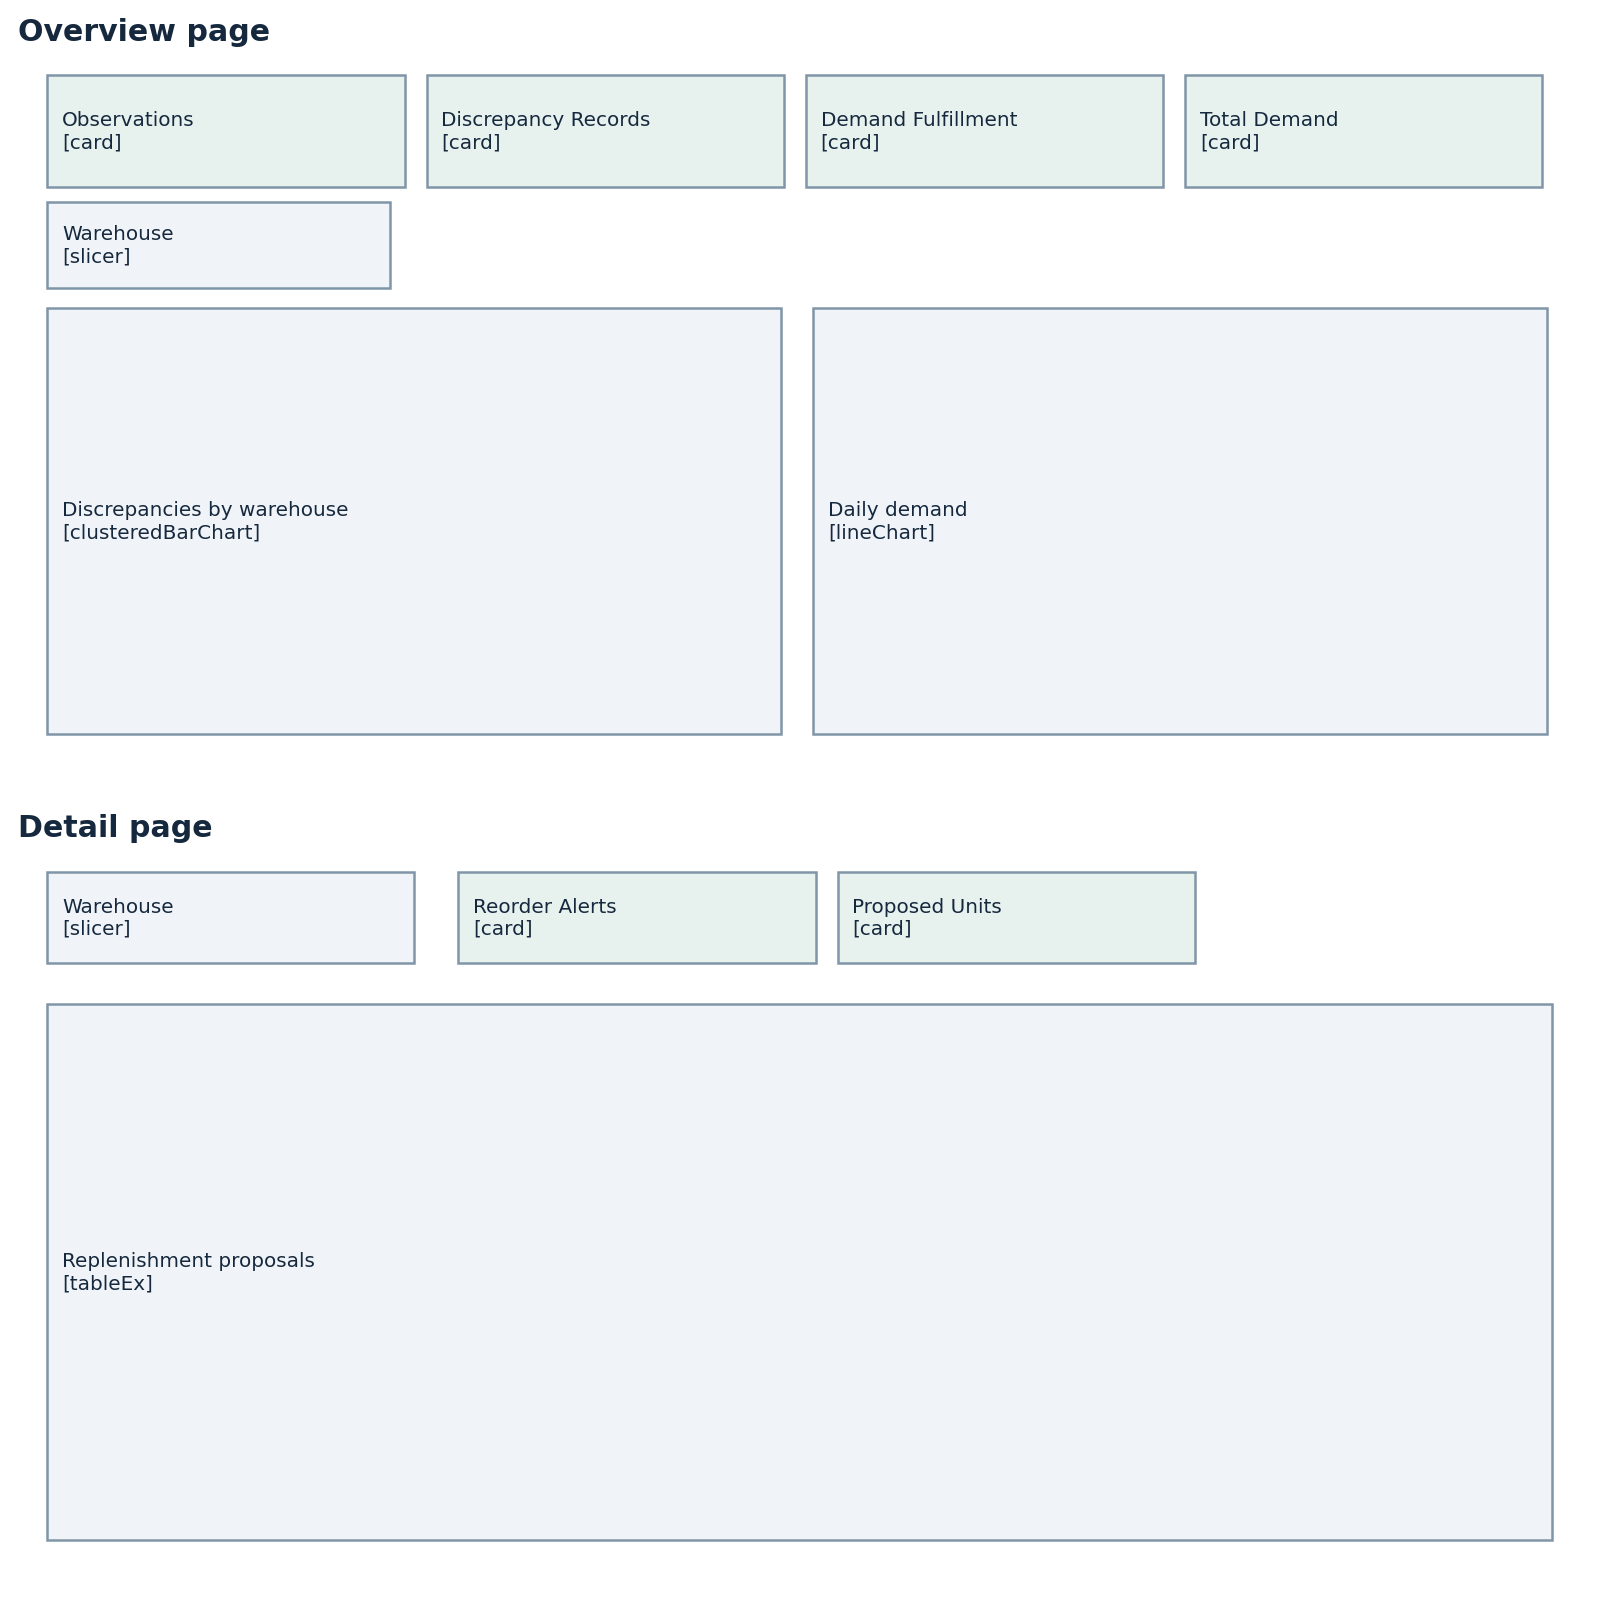
\includegraphics[width=0.90\textwidth,height=0.72\textheight,keepaspectratio]{../../reports/figures/powerbi-layout.png}
\caption{Layout diagram derived from PBIR visual coordinates. This is not a Power BI Desktop screenshot.}\label{fig:powerbi-layout}
\end{figure*}

The package includes a PBIP entry point, PBIR report pages and a TMSL model.bim semantic model \cite{r3,r4,r5}. Power Query decodes an embedded CSV snapshot, promotes headers and applies explicit data types. DAX measures provide aggregation under report filter context. Ratio measures use the DIVIDE function with an explicit alternate result for zero denominators \cite{r6}.


The overview page groups KPI cards, a warehouse slicer and two charts. The detail page exposes replenishment proposals and a separate warehouse slicer. The daily and recommendation tables are independent grains, so each page uses measures from its own table.


Verification boundary: JSON schema and field-reference checks cover the source package. Power BI Desktop rendering, refresh and DAX execution remain outside the present validation scope. The supplied deliverable is editable Power BI project source.


\section{Sensitivity and comparative analysis}

The analysis output is shown in Fig.~\ref{fig:comparison}.

\begin{figure}[!t]
\centering
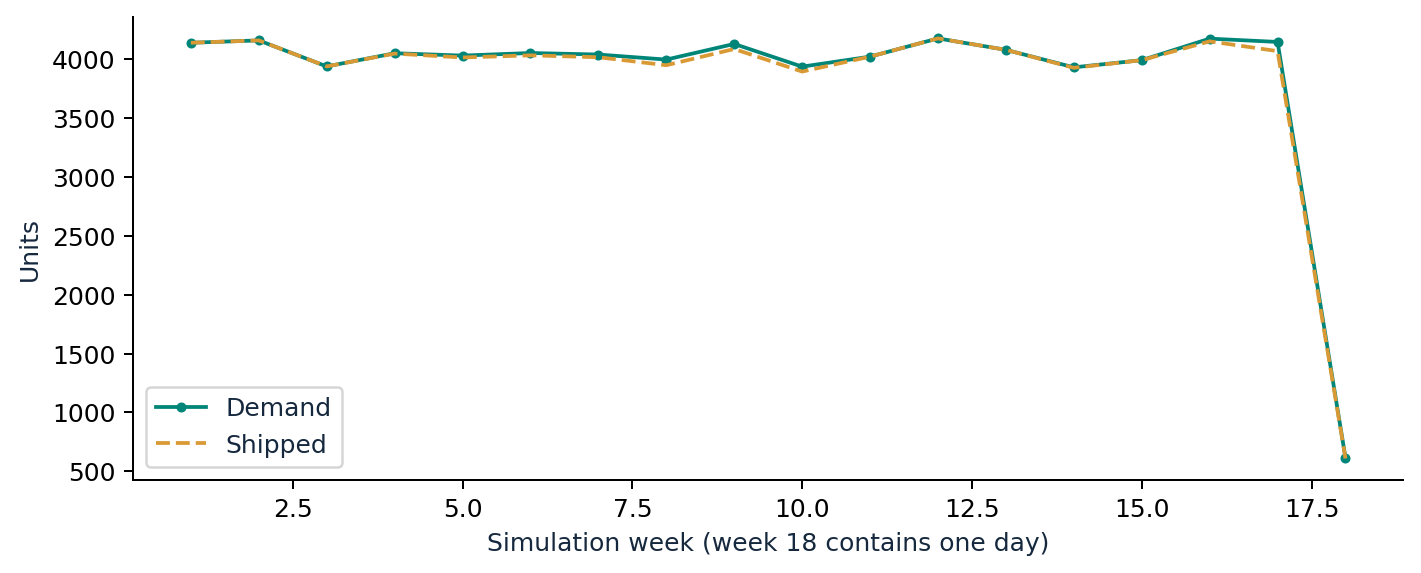
\includegraphics[width=\columnwidth,height=0.25\textheight,keepaspectratio]{../../reports/figures/comparison.png}
\caption{Weekly demand and shipped units. The final period contains only day 120.}\label{fig:comparison}
\end{figure}

Table~\ref{tab:5} summarizes sensitivity results.

\begin{table}[H]
\caption{Sensitivity results}\label{tab:5}
\centering\footnotesize
\setlength{\tabcolsep}{3pt}
\begin{tabularx}{\columnwidth}{>{\raggedright\arraybackslash}X >{\raggedright\arraybackslash}X >{\raggedright\arraybackslash}X}
\hline
\textbf{Lead time (days)} & \textbf{Reorder alerts} & \textbf{Proposed units} \\
\hline
3 & 1 & 280 \\
7 & 2 & 469 \\
10 & 2 & 479 \\
14 & 5 & 836 \\
\hline
\end{tabularx}
\end{table}

With the same closing stock and demand history, increasing lead time from 3 to 14 days increases the alert count from one to five and proposed units from 280 to 836. The 21-day target horizon remains fixed. This isolates the effect of lead-time demand and safety stock.


No service-level improvement is estimated from these proposals because they are not simulated as future receipts. A policy comparison would require a forward simulation with supplier lead-time variation, purchase orders and holding-cost assumptions.


\section{Implementation excerpts}

\subsection{Reorder threshold}

\noindent\begin{minipage}{\columnwidth}
\begin{lstlisting}
def reorder_point(mean_daily_demand, daily_std,
                  lead_time=7, z=1.65):
    if min(mean_daily_demand, daily_std, lead_time, z) < 0:
        raise ValueError("Inputs must be nonnegative")
    return math.ceil(
        mean_daily_demand * lead_time
        + z * daily_std * math.sqrt(lead_time)
    )
\end{lstlisting}
\end{minipage}


Equivalent formatted excerpt of src/run.py. The production function uses the same calculation and rejects negative inputs. The recommendation function adds history selection, target stock and the trigger condition.


\subsection{Stock conservation}

\noindent\begin{minipage}{\columnwidth}
\begin{lstlisting}
shipped = min(erp_stock + received, demand)
erp_stock += received - shipped
wms_stock = max(0, erp_stock + measurement_noise)
\end{lstlisting}
\end{minipage}


The last line illustrates the WMS observation rule. Measurement noise does not change ERP closing stock and is not carried forward as a physical adjustment.


\subsection{Code organization}

src/run.py owns simulation and business rules. src/reporting.py handles CSV and HTML rendering. scripts/analyze.py creates scenario evidence. scripts/build\_powerbi.py regenerates the embedded snapshot and report definitions. Tests exercise calculations, edge cases and report generation.


\section{Validation and reproducibility}

Table~\ref{tab:6} summarizes verification evidence.

\begin{table}[H]
\caption{Verification evidence}\label{tab:6}
\centering\footnotesize
\setlength{\tabcolsep}{3pt}
\begin{tabularx}{\columnwidth}{>{\raggedright\arraybackslash}X >{\raggedright\arraybackslash}X >{\raggedright\arraybackslash}X}
\hline
\textbf{Check} & \textbf{Evidence} & \textbf{Outcome} \\
\hline
Business-rule tests & Stock conservation, reorder examples and invalid inputs & Passed \\
Repeat generation & Same seed and arguments reproduce identical exports & Passed \\
Browser interactions & Warehouse filter, empty search, CSV export, mobile width & Passed \\
Report source & PBIR JSON schema and model-field linkage checks & Passed \\
Desktop Power BI & Windows application, refresh and DAX engine & Not executed \\
\hline
\end{tabularx}
\end{table}

\subsection{Reproduction commands}

\noindent\begin{minipage}{\columnwidth}
\begin{lstlisting}
python src/run.py
python scripts/analyze.py
python scripts/build_powerbi.py
python -m unittest discover -s tests -v
\end{lstlisting}
\end{minipage}


The default analysis uses the Python standard library. The report is compiled from the included IEEEtran LaTeX source using pdfLaTeX. PDF charts and tables draw from committed CSV and JSON outputs. Browser screenshots record the generated HTML interface rather than a hand-drawn imitation.


\subsection{Cross-checks}

All 5,760 rows satisfy ERP stock conservation. Shipments never exceed demand or available ERP stock. The 48-row recommendation table contains one latest proposal per warehouse-SKU pair. Recommended quantity is zero whenever the trigger is false.


\subsection{Scope of assurance}

Passing these checks establishes internal consistency for the stated rules and dataset. It does not establish calibration against a real warehouse, production readiness or economic benefit.


\section{Limitations and conclusion}

\subsection{Model limitations}

\textbullet{} Lead time is fixed and daily demand is treated as independent.


\textbullet{} No open purchase orders, backorders, reservations, MOQ or expiry constraints are modeled.


\textbullet{} WMS variance is injected measurement noise, not an inferred reconciliation cause.


\textbullet{} Proposals are evaluated at one closing snapshot and not executed in the simulation.


\subsection{Next engineering priorities}

An operational extension should introduce validated external data, explicit business definitions, schema checks and exception ownership. A replenishment policy backtest should model order placement, supplier lead times, receipts and total inventory cost.


\subsection{Conclusion}

The project provides an auditable chain from simulated observations to decision fields, exports and visual review. Its main contribution is the separation of stock reconciliation from demand-based replenishment decisions.


The reported outputs are reproducible and the calculation boundaries are documented. Power BI source is supplied as an editable project, with Desktop verification explicitly separated from the automated source checks.


\section{Artifact Availability}

\subsection{Artifact index}

Table~\ref{tab:7} summarizes repository artifacts.

\begin{table}[H]
\caption{Repository artifacts}\label{tab:7}
\centering\footnotesize
\setlength{\tabcolsep}{3pt}
\begin{tabularx}{\columnwidth}{>{\raggedright\arraybackslash}X >{\raggedright\arraybackslash}X}
\hline
\textbf{Path} & \textbf{Purpose} \\
\hline
src/ & Simulation, calculations and HTML reporting \\
reports/*.csv, *.json & Baseline and scenario evidence \\
reports/dashboard.html & Interactive operational dashboard \\
reports/figures/ & Actual browser captures, charts and layout diagram \\
powerbi/ & PBIP, PBIR and semantic model source \\
tests/ & Automated checks \\
docs/methodology.md & Definitions and assumptions \\
reports/project-report.pdf & This technical report \\
\hline
\end{tabularx}
\end{table}

\balance
\begin{thebibliography}{00}

\bibitem{r1} Python Software Foundation. random: Generate pseudo-random numbers. [Online]. Available: \url{https://docs.python.org/3/library/random.html}. Accessed: Oct. 27, 2026.

\bibitem{r2} Python Software Foundation. statistics: Mathematical statistics functions. [Online]. Available: \url{https://docs.python.org/3/library/statistics.html}. Accessed: Oct. 27, 2026.

\bibitem{r3} Microsoft. Power BI Desktop projects. [Online]. Available: \url{https://learn.microsoft.com/en-us/power-bi/developer/projects/projects-overview}. Accessed: Oct. 27, 2026.

\bibitem{r4} Microsoft. Power BI project report folder and PBIR. [Online]. Available: \url{https://learn.microsoft.com/en-us/power-bi/developer/projects/projects-report}. Accessed: Oct. 27, 2026.

\bibitem{r5} Microsoft. Power BI project semantic model folder. [Online]. Available: \url{https://learn.microsoft.com/en-us/power-bi/developer/projects/projects-dataset}. Accessed: Oct. 27, 2026.

\bibitem{r6} Microsoft. DIVIDE function (DAX). [Online]. Available: \url{https://learn.microsoft.com/en-us/dax/divide-function-dax}. Accessed: Oct. 27, 2026.

\end{thebibliography}
\end{document}
